% Template for PLoS
% Version 3.6 Aug 2022
%
% % % % % % % % % % % % % % % % % % % % % %
%
% -- IMPORTANT NOTE
%
% This template contains comments intended 
% to minimize problems and delays during our production 
% process. Please follow the template instructions
% whenever possible.
%
% % % % % % % % % % % % % % % % % % % % % % % 
%
% Once your paper is accepted for publication, 
% PLEASE REMOVE ALL TRACKED CHANGES in this file 
% and leave only the final text of your manuscript. 
% PLOS recommends the use of latexdiff to track changes during review, as this will help to maintain a clean tex file.
% Visit https://www.ctan.org/pkg/latexdiff?lang=en for info or contact us at latex@plos.org.
%
%
% There are no restrictions on package use within the LaTeX files except that no packages listed in the template may be deleted.
%
% Please do not include colors or graphics in the text.
%
% The manuscript LaTeX source should be contained within a single file (do not use \input, \externaldocument, or similar commands).
%
% % % % % % % % % % % % % % % % % % % % % % %
%
% -- FIGURES AND TABLES
%
% Please include tables/figure captions directly after the paragraph where they are first cited in the text.
%
% DO NOT INCLUDE GRAPHICS IN YOUR MANUSCRIPT
% - Figures should be uploaded separately from your manuscript file. 
% - Figures generated using LaTeX should be extracted and removed from the PDF before submission. 
% - Figures containing multiple panels/subfigures must be combined into one image file before submission.
% For figure citations, please use "Fig" instead of "Figure".
% See http://journals.plos.org/plosone/s/figures for PLOS figure guidelines.
%
% Tables should be cell-based and may not contain:
% - spacing/line breaks within cells to alter layout or alignment
% - do not nest tabular environments (no tabular environments within tabular environments)
% - no graphics or colored text (cell background color/shading OK)
% See http://journals.plos.org/plosone/s/tables for table guidelines.
%
% For tables that exceed the width of the text column, use the adjustwidth environment as illustrated in the example table in text below.
%
% % % % % % % % % % % % % % % % % % % % % % % %
%
% -- EQUATIONS, MATH SYMBOLS, SUBSCRIPTS, AND SUPERSCRIPTS
%
% IMPORTANT
% Below are a few tips to help format your equations and other special characters according to our specifications. For more tips to help reduce the possibility of formatting errors during conversion, please see our LaTeX guidelines at http://journals.plos.org/plosone/s/latex
%
% For inline equations, please be sure to include all portions of an equation in the math environment.  For example, x$^2$ is incorrect; this should be formatted as $x^2$ (or $\mathrm{x}^2$ if the romanized font is desired).
%
% Do not include text that is not math in the math environment. For example, CO2 should be written as CO\textsubscript{2} instead of CO$_2$.
%
% Please add line breaks to long display equations when possible in order to fit size of the column. 
%
% For inline equations, please do not include punctuation (commas, etc) within the math environment unless this is part of the equation.
%
% When adding superscript or subscripts outside of brackets/braces, please group using {}.  For example, change "[U(D,E,\gamma)]^2" to "{[U(D,E,\gamma)]}^2". 
%
% Do not use \cal for caligraphic font.  Instead, use \mathcal{}
%
% % % % % % % % % % % % % % % % % % % % % % % % 
%
% Please contact latex@plos.org with any questions.
%
% % % % % % % % % % % % % % % % % % % % % % % %

\documentclass[10pt,letterpaper]{article}
\usepackage[top=0.85in,left=2.75in,footskip=0.75in]{geometry}

% amsmath and amssymb packages, useful for mathematical formulas and symbols
\usepackage{amsmath,amssymb}

% Use adjustwidth environment to exceed column width (see example table in text)
\usepackage{changepage}

% textcomp package and marvosym package for additional characters
\usepackage{textcomp,marvosym}

% cite package, to clean up citations in the main text. Do not remove.
% \usepackage{cite}

% Use nameref to cite supporting information files (see Supporting Information section for more info)
\usepackage{nameref,hyperref}

% line numbers
\usepackage[right]{lineno}

% ligatures disabled
\usepackage[nopatch=eqnum]{microtype}
\DisableLigatures[f]{encoding = *, family = * }

% color can be used to apply background shading to table cells only
\usepackage[table]{xcolor}

% array package and thick rules for tables
\usepackage{array}

% create "+" rule type for thick vertical lines
\newcolumntype{+}{!{\vrule width 2pt}}

% create \thickcline for thick horizontal lines of variable length
\newlength\savedwidth
\newcommand\thickcline[1]{%
  \noalign{\global\savedwidth\arrayrulewidth\global\arrayrulewidth 2pt}%
  \cline{#1}%
  \noalign{\vskip\arrayrulewidth}%
  \noalign{\global\arrayrulewidth\savedwidth}%
}

% \thickhline command for thick horizontal lines that span the table
\newcommand\thickhline{\noalign{\global\savedwidth\arrayrulewidth\global\arrayrulewidth 2pt}%
\hline
\noalign{\global\arrayrulewidth\savedwidth}}


% Remove comment for double spacing
%\usepackage{setspace} 
%\doublespacing

% Text layout
\raggedright
\setlength{\parindent}{0.5cm}
\textwidth 5.25in 
\textheight 8.75in

% Bold the 'Figure #' in the caption and separate it from the title/caption with a period
% Captions will be left justified
\usepackage[aboveskip=1pt,labelfont=bf,labelsep=period,justification=raggedright,singlelinecheck=off]{caption}
\renewcommand{\figurename}{Fig}

% Use the PLoS provided BiBTeX style
% \bibliographystyle{plos2015}
% Remove brackets from numbering in List of References

\makeatletter
\renewcommand{\@biblabel}[1]{\quad#1.}
\makeatother
  


% Header and Footer with logo
\usepackage{lastpage,fancyhdr,graphicx}
\usepackage{epstopdf}
\usepackage{biblatex}
\addbibresource{Mendeley.bib}
\addbibresource{manual.bib}

%\pagestyle{myheadings}
\pagestyle{fancy}
\fancyhf{}
%\setlength{\headheight}{27.023pt}
%\lhead{\includegraphics[width=2.0in]{PLOS-submission.eps}}
\rfoot{\thepage/\pageref{LastPage}}
\renewcommand{\headrulewidth}{0pt}
\renewcommand{\footrule}{\hrule height 2pt \vspace{2mm}}
\fancyheadoffset[L]{2.25in}
\fancyfootoffset[L]{2.25in}
\lfoot{\today}

%% Include all macros below

\newcommand{\lorem}{{\bf LOREM}}
\newcommand{\ipsum}{{\bf IPSUM}}

%% END MACROS SECTION


\begin{document}
\vspace*{0.2in}

% Title must be 250 characters or less.
\begin{flushleft}
{\Large
\textbf\newline{Effects of multistability, absorbing boundaries and growth on Turing pattern formation} % Please use "sentence case" for title and headings (capitalize only the first word in a title (or heading), the first word in a subtitle (or subheading), and any proper nouns).
}
\newline
% Insert author names, affiliations and corresponding author email (do not include titles, positions, or degrees).
\\
Martina Oliver Huidobro \textsuperscript{1},
Robert G. Endres \textsuperscript{1}


\bigskip
\textbf{1} Life Sciences Department, Imperial College London, UK
\\
\bigskip

% Insert additional author notes using the symbols described below. Insert symbol callouts after author names as necessary.
% 
% Remove or comment out the author notes below if they aren't used.
%
% Primary Equal Contribution Note
\Yinyang These authors contributed equally to this work.

% Additional Equal Contribution Note
% Also use this double-dagger symbol for special authorship notes, such as senior authorship.
\ddag These authors also contributed equally to this work.

% Current address notes
\textcurrency Current Address: Dept/Program/Center, Institution Name, City, State, Country % change symbol to "\textcurrency a" if more than one current address note
% \textcurrency b Insert second current address 
% \textcurrency c Insert third current address

% Deceased author note
\dag Deceased

% Group/Consortium Author Note
\textpilcrow Membership list can be found in the Acknowledgments section.

% Use the asterisk to denote corresponding authorship and provide email address in note below.
* correspondingauthor@institute.edu

\end{flushleft}
% Please keep the abstract below 300 words
\section*{Abstract}



% Please keep the Author Summary between 150 and 200 words
% Use first person. PLOS ONE authors please skip this step. 
% Author Summary not valid for PLOS ONE submissions.   
\section*{Author summary}


\linenumbers

% Use "Eq" instead of "Equation" for equation citations.
\section*{Introduction}


% Place figure captions after the first paragraph in which they are cited.
\begin{figure}[!h]
    \includegraphics[width=1\textwidth]{figures/biological_example}

    \caption{{\bf Bold the figure title.}
        Figure caption text here, please use this space for the figure panel descriptions instead of using subfigure commands. A: Lorem ipsum dolor sit amet. B: Consectetur adipiscing elit.}
    \label{fig1}
\end{figure}











%\begin{eqnarray}
%\label{eq:schemeP}
%	\mathrm{P_Y} = \underbrace{H(Y_n) - H(Y_n|\mathbf{V}^{Y}_{n})}_{S_Y} + \underbrace{H(Y_n|\mathbf{V}^{Y}_{n})- H(Y_n|\mathbf{V}^{X,Y}_{n})}_{T_{X\rightarrow Y}},
%\end{eqnarray}

\section*{Materials and methods}

\subsection*{Linear stability analysis}

% For figure citations, please use "Fig" instead of "Figure". \nameref{S1_Video}


\subsection*{Numerical methods}



\subsection*{Classification methods}



% Results and Discussion can be combined.
\section*{Results}
\subsection*{Multistability in Turing}

In this section, we demonstrate how linear stability analysis is not sufficient or necessary to predict Turing patterns (TPs) in multi-stable systems.
In particular, we study in detail the dynamical behaviour of multi-stable systems during pattern formation, which will lead to the creation or breaking of the pattern.
The motivation behind this arises from the high degree of multistability exhibited by biological systems, where cell-fate decisions have to be taken within this landscape ~\parencite{huang2000shape,moris2016transition}.
Multistability is especially common in systems with non-linearities and feedback loops, as the ones in biology or in our models~\parencite{pham2020complexity, leite2009multistability}.

Using the two-node non-linear Turing topology (Eq. \ref{eq:turinghill}), multi-stable solutions were found and studied to understand how the patterning dynamics get affected when multiple steady-state solutions are found.
First, LSA is carried out on particular parameter sets to find multiple steady states with different stability nature (e.g.~stable, unstable, Turing I, Turing I-Hopf).
Then numerical simulations are computed where the initial condition is a random uniform distribution around a particular steady state.
Different pattern outcomes result depending on where in the phase diagram the initial condition is.
Following the classical hypothesis used in the Turing robustness literature, we would expect stable and unstable systems to not produce patterns and Turing to produce patterns.
Here, we present various examples of how this hypothesis can break under multistability conditions.

Fig.~\ref{fig:fig1} shows a case where diffusion-driven instability conditions are not required for Turing pattern formation.
The unstable state, having a dispersion relation with a peak below zero (Fig.~\ref{fig:fig1}C), managed to get into a Turing pattern regime as it is attracted by the neighbouring Turing steady state.
It therefore produces a stationary pattern (Fig.~\ref{fig:fig1}B), even though its dispersion relation does not predict so.
This trajectory is depicted in the phase diagram (Fig.~\ref{fig:fig1}A) which shows the steady states along with the vector field to understand the potential trajectories of the system.
The phase diagram does not fully capture the dynamics as it describes the system without diffusion, while the dispersion relation and the numerical solution do consider diffusion.

\begin{figure}[!h]
    \includegraphics[width=1\textwidth]{figures/multistability1}

    \caption{{\bf Stationary Patterns in multistability.} \textbf{(A)} Phase diagram without diffusion illustrating three distinct steady states where the derivative is zero: stable, unstable, and stable (Turing). These steady states are represented within a parameter space defined by two axes: concentrations of A and I. The vector field, indicated by light green arrows, shows the direction of the derivatives of the system at various points in the parameter space. A hand-drawn trajectory is also shown (dark green arrow), demonstrating how the unstable state may evolve into the Turing state. \textbf{(B)} Dispersion relation showing each type of state. \textbf{(C)} Numerical solutions of the three steady states with diffusion, where the unstable state unexpectedly produces a Turing-like stationary pattern.}
    \label{fig2}
\end{figure}


Then, we present a case where LSA incorrectly predicts stationary pattern formation.
Fig.~\ref{fig:fig2} shows an ephemeral or transient pattern that occurs in the unstable and Turing regimes.
The TP initially develops in the vicinity of the Turing steady state.
As the spatial heterogeneity is amplified and settles, it gets attracted by the stable steady state leading to the disruption of the pattern.
This type of transient pattern behaviour has also been recently reported in~\cite{Krause2023}.





\begin{figure}[!h]
    \includegraphics[width=1\textwidth]{figures/multistability2}

    \caption{{\bf Ephemeral patterns in multistability.}
        \textbf{(A)} Phase diagram without diffusion illustrating three distinct steady states where the derivative is zero. The hand-drawn trajectory (dark green arrow) shows an unstable state evolving into a stable (Turing), and a stable (Turing) evolving into a stable. \textbf{(B)} Dispersion relation showing each type of state. \textbf{(C)} Numerical solutions of three steady states with diffusion. Unstable and Turing produce temporary periodic stationary patterns, that then disappear and become spatially homogeneous solutions.}
    \label{fig3}
\end{figure}



% Other interesting examples can be found, for example, where an unstable state is surrounded by two Turing states, this unstable state will robustly lead to a Turing pattern (Fig.~\ref{fig:multistability_leftover}A).
% Additionally, in some cases, the unstable system settles into Turing, but the Turing system gets pulled by the stable attractor (Fig.~\ref{fig:multistability_leftover}B). Additionally, some systems even exhibit three solutions which are homogeneous in time and space (Fig.~\ref{fig:multistability_leftover}C).
% In this case, it would be worth investigating earlier time points with more resolution, as a pattern might appear then.
% Interesting interactions similarly occur with multistability involving Turing I-Hopf solutions which will be mentioned in the following sections (Fig.~\ref{fig:multistability_leftover}D).

%TODO comment on other examples on supplementary 







\subsection*{Beyond the classical dispersion relation}
Multi-stable systems are not the only case where the classical Turing instability theory fails to predict pattern formation.
Other types of dispersion relations beyond classical Turing instabilities can produce stationary patterns and non-stationary regular patterns that might be of interest in developmental biology.
This section aims to document what type of dispersion relations in mono-stable systems can be linked to what type of patterns, to gain insights into predicting pattern formation from linear stability analysis.
We will first present a classification for the different types of dispersion relations.
Subsequently, we will show the classification for the different types of pattern outcomes, where the system is defined in a non-growing domain with reflective boundary conditions (Neumann, where the derivative is zero at the boundary).
Finally, we will reconstruct the 2x2 confusion matrix (Fig.~\ref{fig:lsa_numerical_confusion_literature}) currently used as an assumption in the literature, to show a more complete view on how to interpret dispersion relations.
The new confusion matrix will show more types of dispersion relation and more pattern outcomes leading to a 5x4 confusion matrix.

First, we classify the different dispersion relations obtained from LSA into 5 types:

% \begin{itemize}
%     \item Stable dispersion relations (Fig~\ref{fig:fig4}A) have all eigenvalues $\sigma$ below zero for any wavenumber $k_{n}$.
%     \item Unstable dispersion relations (Fig~\ref{fig:fig4}B) have a positive eigenvalue at $k_{0}=0$ which eventually drops below zero as diffusion is introduced (i.e. $k_{n}>0$).
%     \item Hopf-type dispersion relations, as with any unstable dispersion relation, shows an instability without diffusion ($\sigma>0$ for $k_{0}=0$) which eventually drops below zero for positive wavenumbers.
% However, in the case of the Hopf-type dispersion relation, when the eigenvalues cross the zero line, there is a pair of complex conjugate eigenvalues (Fig~\ref{fig:fig4}C).
% A Hopf-like dispersion relation is different to a Hopf bifurcation: a bifurcation displays a shift in stability as a model parameter changes, while the Hopf-like dispersion is a change in stability as a function of the wavenumber $k_{n}$.
% %In this case, the bifurcation parameter would be $k$, making the system go from unstable to stable by changing this parameter.
% \item Turing I dispersion relations, as previously mentioned, are stable without diffusion, have an instability for a positive wavenumber, and finally become stable again for very large wavenumbers (Fig~\ref{fig:fig4}D).
% \item Turing I-Hopf dispersion relations, are a combination of Turing I and Hopf-type dispersion relations.
% As the Hopf-type dispersion, they are unstable without diffusion.
% Then, as $k_{n}$ is increased, the system becomes stable with a pair of complex conjugates as the eigenvalues cross the zero line.
% Finally, a Turing I-type behaviour arises getting a peak above zero and decaying again for large wavenumbers (Fig~\ref{fig:fig4}E).
% \end{itemize}

Other types of dispersion relation exist which are not displayed here such as Turing II, where the eigenvalues do not become stable again for very large wavenumbers.
Therefore, this system displays an instability at very large wavenumbers which results in infinitesimally small wavelength patterns.
These are considered to produce homogeneous solutions, except in the case of space discretization where they can produce small wavelength patterns~\parencite{Wang2022}.
However, Turing II solutions are not possible in systems such as this one where all nodes are diffusing.
This is because for $k_n \rightarrow \inf$, all eigenvalues $\sigma$ must be negative (see Eq.~\ref{jacobian_diffusion}).

% \begin{figure}[!h]
%     \includegraphics[width=1\textwidth]{figures/dispersion}

%     \caption{{\bf Different types of dispersion relation.}
%         Dispersion relation shows the eigenvalue as a function of wavenumber. The continuous line represents the real part, while the dotted line represents the imaginary part. \textbf{(A) Stable:} all eigenvalues are below zero. \textbf{(B) Unstable:} eigenvalues at $k_{n}$=0 are positive meaning the system is unstable without diffusion. \textbf{(C) Hopf:}~unstable type, with hopf bifurcation for parameter wavenumber $k_{n}$. For a certain $k_{n}$, the system flips from unstable to stable, crossing the zero eigenvalue line. At the crossing, there is a pair of complex conjugate eigenvalues. \textbf{(D) Turing I:} the dispersion shows a diffusion driven instability. At $k_{n}$=0, the system is stable and has negative eigenvalues. As diffusion is introduced, $k_{n}$>0, the system becomes unstable and stable again for high $k$ values. \textbf{(E) Turing I-Hopf:} a combination of Turing I and Hopf, meaning the system starts as a Hopf with a positive eigenvalue at $k_{n}$=0, then the system transitions to stable with a pair of complex conjugates. Finally, there is a dispersion peak characteristic of Turing that drops for high values of $k$.}
%     \label{fig4}
% \end{figure}


As with the classification of the dispersion relations, we develop a method to classify the patterns produced numerically into homogeneous, temporal oscillator, non-stationary pattern and stationary pattern.
By classifying both LSA and numerical outputs, we can generate a new confusion matrix with information about other types of dispersion relations and other types of spatio-temporal patterns.

We use a decision tree for the classification where the two layers are spatial homogeneity and convergence in time, as seen in Fig.~\ref{fig:no growth classification}.
This decision tree leads to the 4 types of patterns mentioned.
A pattern will be considered spatially homogeneous if the final snapshot $U$ for any of the two molecular species fulfils the following condition
\begin{equation}
    \frac{max(U) - min(U)}{max(U)} \leq 0.01
\end{equation}
A pattern will be considered converged if the last 30 time points for any of the two molecular species fulfils the following condition
\begin{equation}
    \frac{max(U[-30:]) - min(U[-30:])}{max(U[-30:])} \leq 0.05
\end{equation}
The thresholds chosen were fine-tuned by testing them on the numerical patterns to obtain the best classification results.
Using these two characteristics, spatial homogeneity and convergence, we can obtain 4 classes of patterns as seen in Fig.~\ref{fig:no growth classification}:
 
% \begin{itemize}
%     \item Homogeneous patterns are homogeneous in space and converge in time.
%     \item Temporal oscillators, also called limit cycles, are homogeneous in space but do not converge, as they oscillate in time.
%     \item Non-stationary patterns are not homogeneous in space and do not converge in time.
%     \item Finally, Stationary patterns are not homogeneous in space but converge in time.
% \end{itemize}

% \begin{itemize}
% 	\item First bulleted item.
% 	\item Second bulleted item.
% 	\item Third bulleted item.
% \end{itemize}

% \begin{figure}[H] % h! is a placement specifier; it tries to place the image here.
%     \centering
%     \begin{adjustbox}{center}
%     \includegraphics[width=1\textwidth]{chapters/Chapter 1/no growth classification} % The name of your image file; assumes it is in the same directory as your .tex file
%     \end{adjustbox}
%     \caption{\textbf{Decision tree for pattern classification in non-growing domains with reflective boundaries}. A decision tree is based on two layers: spatial homogeneity and convergence. The numerical solutions for the four different pattern outcomes including a homogeneous, temporal oscillator, non-stationary pattern and stationary pattern are shown below.}
%     \label{fig:no growth classification} % A label for referencing this figure later in the document
% \end{figure}


High-throughput studies like~\cite{Scholes2019, Zheng2016, Marcon} only consider Turing I as patterning and the rest is discarded.
Here, we explore beyond Turing I and stationary patterns to give a more complete view of the relationship between linear stability and spatio-temporal patterns.
9,087 parameter sets are analysed from the non-linear Turing model (Eqs. \ref{eq:turinghill}) to obtain dispersion relations and numerical patterns.
Because systems such as Turing and Turing I-Hopf are undersampled in the parameter space, the dataset is enriched with them to ensure we capture enough distinct dynamical behaviours.
Multi-stable systems are not included in this analysis to understand the direct relationships between the dispersion relation and numerics.
The two types of classifications described above are applied, and a new 5x4 confusion matrix is generated (Fig.~\ref{fig:lsa_numerical_confusion}).



It is worth pointing out some interesting examples obtained from this confusion matrix.
For example, Turing I-Hopf seems to lead to stationary patterns often (see Fig.~\ref{fig:interesting_cases_nogrowth}A), meaning they would need to be investigated in high-throughput robustness studies.
The production of periodic patterns by Turing I-Hopf instabilities has been already documented in the literature~\cite{Liu2007}.
Some unstable dispersion relations can also lead to stationary patterns (see Fig.~\ref{fig:interesting_cases_nogrowth}B).
Additionally, Hopf solutions display interesting non-stationary patterns (see Fig.~\ref{fig:interesting_cases_nogrowth}C).
Unfortunately, some Hopf solutions are misclassified as Stationary patterns (see Fig.~\ref{fig:interesting_cases_nogrowth}D) due to an inadequate threshold of the convergence classification.
In this specific case, a higher window than 30 should be taken when considering convergence and a higher threshold for homogeneity.
It is important to understand that this is an initial exploratory analysis where misclassification might occur.
This is because of the difficulty of setting common thresholds for a wide variety of numerical solutions with different wavelengths, time scales and dynamic ranges.




\subsection*{Investigating boundaries and growth}

\begin{figure}[!h] 
    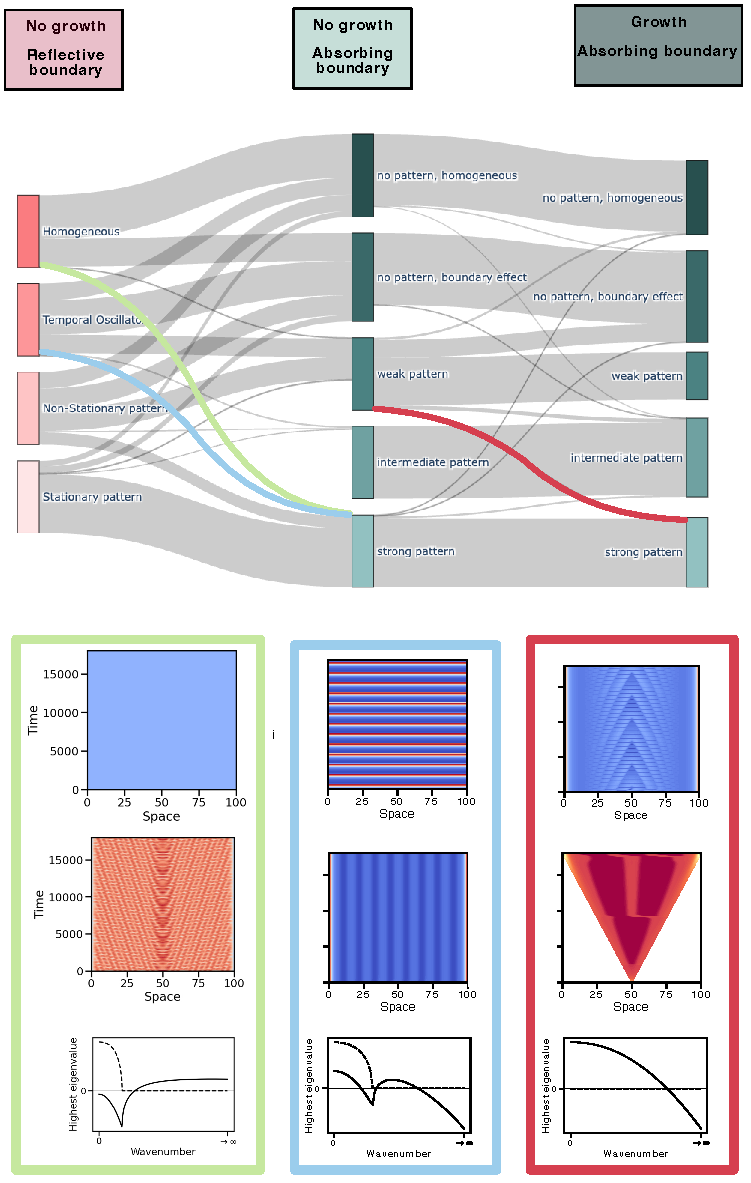
\includegraphics[width=1\textwidth]{figures/boundaries_growth}

    \caption{{\bf Bold the figure title.}
       }
    \label{fig5}
\end{figure}
%% Place tables after the first paragraph in which they are cited.
%\begin{table}[!ht]
%\begin{adjustwidth}{-2.25in}{0in} % Comment out/remove adjustwidth environment if table fits in text column.
%\centering
%\caption{
%{\bf Table caption Nulla mi mi, venenatis sed ipsum varius, volutpat euismod diam.}}
%\begin{tabular}{|l+l|l|l|l|l|l|l|}
%\hline
%\multicolumn{4}{|l|}{\bf Heading1} & \multicolumn{4}{|l|}{\bf Heading2}\\ \thickhline
%$cell1 row1$ & cell2 row 1 & cell3 row 1 & cell4 row 1 & cell5 row 1 & cell6 row 1 & cell7 row 1 & cell8 row 1\\ \hline
%$cell1 row2$ & cell2 row 2 & cell3 row 2 & cell4 row 2 & cell5 row 2 & cell6 row 2 & cell7 row 2 & cell8 row 2\\ \hline
%$cell1 row3$ & cell2 row 3 & cell3 row 3 & cell4 row 3 & cell5 row 3 & cell6 row 3 & cell7 row 3 & cell8 row 3\\ \hline
%\end{tabular}
%\begin{flushleft} Table notes Phasellus venenatis, tortor nec vestibulum mattis, massa tortor interdum felis, nec pellentesque metus tortor nec nisl. Ut ornare mauris tellus, vel dapibus arcu suscipit sed.
%\end{flushleft}
%\label{table1}
%\end{adjustwidth}
%\end{table}


\subsection*{Multistability in Turing}


\subsection*{Sed ac quam id nisi malesuada congue}



\section*{Discussion}


\section*{Conclusion}


\section*{Supporting information}

% Include only the SI item label in the paragraph heading. Use the \nameref{label} command to cite SI items in the text.
\paragraph*{S1 Fig.}
\label{S1_Fig}
{\bf Bold the title sentence.} Add descriptive text after the title of the item (optional).

\paragraph*{S2 Fig.}
\label{S2_Fig}
{\bf Lorem ipsum.} Maecenas convallis mauris sit amet sem ultrices gravida. Etiam eget sapien nibh. Sed ac ipsum eget enim egestas ullamcorper nec euismod ligula. Curabitur fringilla pulvinar lectus consectetur pellentesque.

\paragraph*{S1 File.}
\label{S1_File}
{\bf Lorem ipsum.}  Maecenas convallis mauris sit amet sem ultrices gravida. Etiam eget sapien nibh. Sed ac ipsum eget enim egestas ullamcorper nec euismod ligula. Curabitur fringilla pulvinar lectus consectetur pellentesque.

\paragraph*{S1 Video.}
\label{S1_Video}
{\bf Lorem ipsum.}  Maecenas convallis mauris sit amet sem ultrices gravida. Etiam eget sapien nibh. Sed ac ipsum eget enim egestas ullamcorper nec euismod ligula. Curabitur fringilla pulvinar lectus consectetur pellentesque.

\paragraph*{S1 Appendix.}
\label{S1_Appendix}
{\bf Lorem ipsum.} Maecenas convallis mauris sit amet sem ultrices gravida. Etiam eget sapien nibh. Sed ac ipsum eget enim egestas ullamcorper nec euismod ligula. Curabitur fringilla pulvinar lectus consectetur pellentesque.

\paragraph*{S1 Table.}
\label{S1_Table}
{\bf Lorem ipsum.} Maecenas convallis mauris sit amet sem ultrices gravida. Etiam eget sapien nibh. Sed ac ipsum eget enim egestas ullamcorper nec euismod ligula. Curabitur fringilla pulvinar lectus consectetur pellentesque.

\section*{Acknowledgments}
Cras egestas velit mauris, eu mollis turpis pellentesque sit amet. Interdum et malesuada fames ac ante ipsum primis in faucibus. Nam id pretium nisi. Sed ac quam id nisi malesuada congue. Sed interdum aliquet augue, at pellentesque quam rhoncus vitae.

\nolinenumbers

% Either type in your references using
% \begin{thebibliography}{}
% \bibitem{}
% Text
% \end{thebibliography}
%
% or
%
% Compile your BiBTeX database using our plos2015.bst
% style file and paste the contents of your .bbl file
% here. See http://journals.plos.org/plosone/s/latex for 
% step-by-step instructions.
% 
\begin{thebibliography}{10}

\bibitem{bib1}
Conant GC, Wolfe KH.
\newblock {{T}urning a hobby into a job: how duplicated genes find new
  functions}.
\newblock Nat Rev Genet. 2008 Dec;9(12):938--950.

\bibitem{bib2}
Ohno S.
\newblock Evolution by gene duplication.
\newblock London: George Alien \& Unwin Ltd. Berlin, Heidelberg and New York:
  Springer-Verlag.; 1970.

\bibitem{bib3}
Magwire MM, Bayer F, Webster CL, Cao C, Jiggins FM.
\newblock {{S}uccessive increases in the resistance of {D}rosophila to viral
  infection through a transposon insertion followed by a {D}uplication}.
\newblock PLoS Genet. 2011 Oct;7(10):e1002337.

\end{thebibliography}



\end{document}

